\documentclass[11pt]{article}
\title{\textbf{CS 361 Spring 2018\\Homework 11}}
\author{Nathaniel Murphy (njmurph3)}
\date{}

\usepackage{a4wide}
\usepackage{amsfonts}
\usepackage{amsmath}
\usepackage{amsthm}
\usepackage{graphicx}
\usepackage{tikz}
\usepackage[margin=0.5in]{geometry}
\usetikzlibrary{automata,positioning}

\begin{document}
\maketitle
\section*{a)}
I approached the first problem by drawing a FSM with two states. This drawing is provided below along with the transition probabilities and emission probabilities. After modeling this using HMM's Multinomial class, I was able to sample this distribution 100000 times. We see that the probability that the emitted probability is a 1 is approximately 0.193, which is slightly higher than $\frac{1}{6}$. The other values had probability slightly below $\frac{1}{6}$, which is attributed to the lower probability on the unfair die. \\ \\
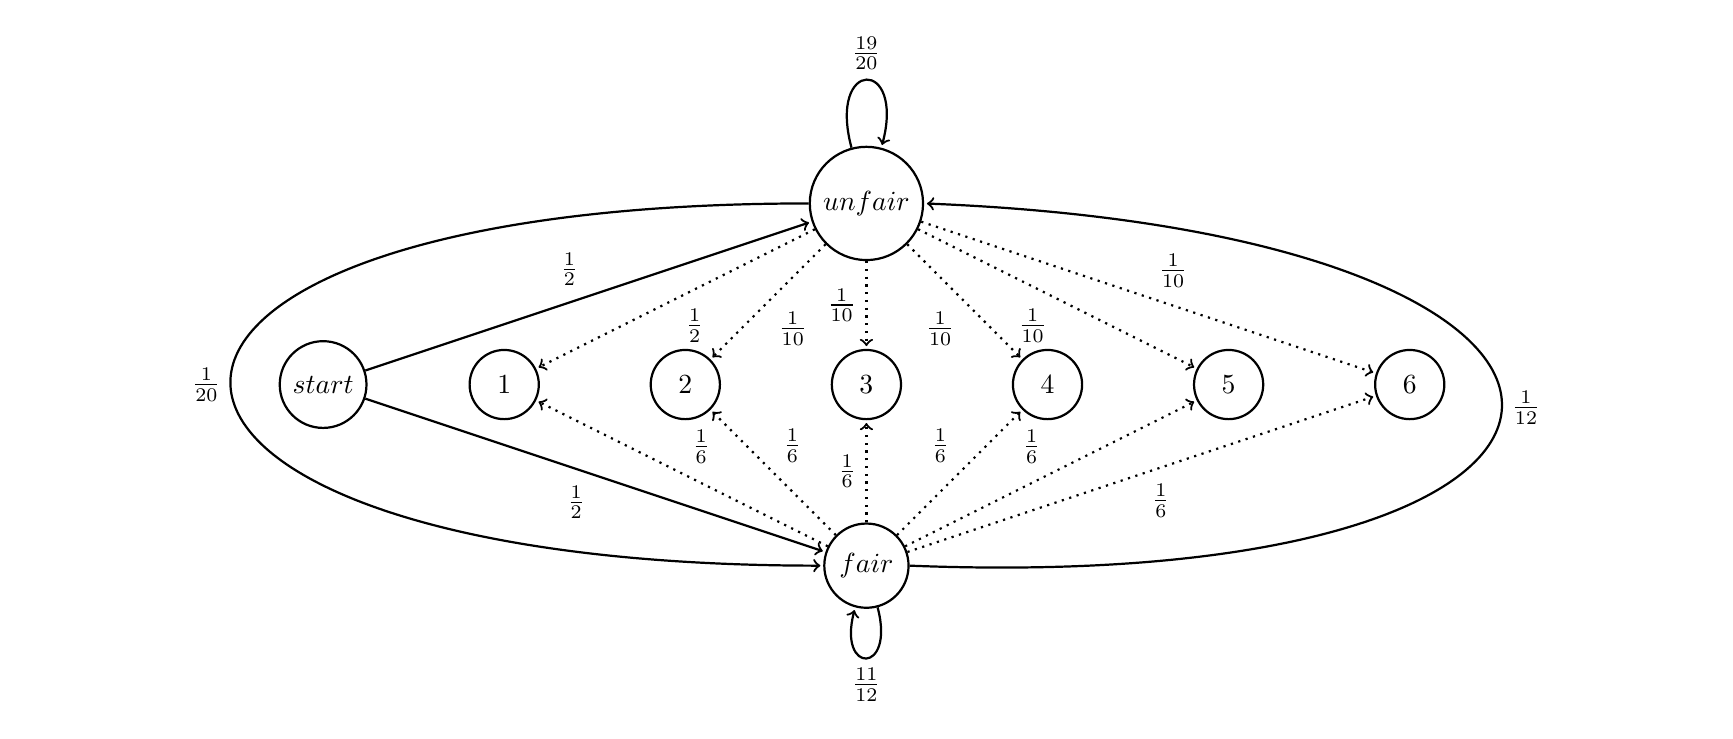
\begin{tikzpicture}[->,shorten >=1pt,auto,on grid,node distance=2.3cm, thick,node/.style={circle,draw}]
	\node[state] (start)   {$start$};
	\node[state] (one) [right=of start] {$1$};
	\node[state] (two) [right=of one] {$2$}; 
	\node[state] (three) [right=of two] {$3$};
	\node[state] (four) [right=of three] {$4$};
	\node[state] (five) [right=of four] {$5$};
	\node[state] (six) [right=of five] {$6$};
	\node[state] (fair) [below=of three] {$fair$}; 
	\node[state] (unfair) [above=of three] {$unfair$};
    \path[->] 
    (start) edge node [swap] {$\frac{1}{2}$} (fair)
		edge node {$\frac{1}{2}$} (unfair)
    (unfair) edge [dotted] node {$\frac{1}{2}$} (one)
    		edge [dotted] node {$\frac{1}{10}$} (two)
    		edge [dotted] node [swap] {$\frac{1}{10}$} (three)
    		edge [dotted] node [swap] {$\frac{1}{10}$} (four)
    		edge [dotted] node [swap] {$\frac{1}{10}$} (five)
    		edge [dotted] node {$\frac{1}{10}$} (six)
    		edge [loop above] node {$\frac{19}{20}$} (unfair)
    		edge [out=180, in=180, looseness=5.5] node [swap] {$\frac{1}{20}$} (fair)
	(fair) edge [dotted] node [swap] {$\frac{1}{6}$} (one)
		edge [dotted] node [swap] {$\frac{1}{6}$} (two)
		edge [dotted] node {$\frac{1}{6}$} (three)
		edge [dotted] node {$\frac{1}{6}$} (four)
		edge [dotted] node {$\frac{1}{6}$} (five)
		edge [dotted] node [swap] {$\frac{1}{6}$} (six)
		edge [bend right=90, looseness=5.5] node [swap] {$\frac{1}{12}$} (unfair)
		edge [loop below] node {$\frac{11}{12}$} (fair)
		
          ;
\end{tikzpicture}
\section*{b)}
For this problem, I simulated draws of 10, 100, 1000, 10000, each 10 times and used MulinomialHMM.decode to predict what the original sequence states were given the sample that I drew. Once I had the predicted states and the true states, I could just count in how many places they varied. I recorded this for each of the 10 epochs and then averaged the accuracies. It looks like sampling a larger number of points did not help accuracy, as it was almost a constant 0.915 throughout all epochs of the simulation.
\end{document}